\section{eo\-Select\-Number$<$ EOT $>$ Class Template Reference}
\label{classeo_select_number}\index{eoSelectNumber@{eoSelectNumber}}
eo\-Select\-Number selects many individuals using {\bf eo\-Select\-One}{\rm (p.\,\pageref{classeo_select_one})} as it's mechanism.  


{\tt \#include $<$eo\-Select\-Number.h$>$}

Inheritance diagram for eo\-Select\-Number$<$ EOT $>$::\begin{figure}[H]
\begin{center}
\leavevmode
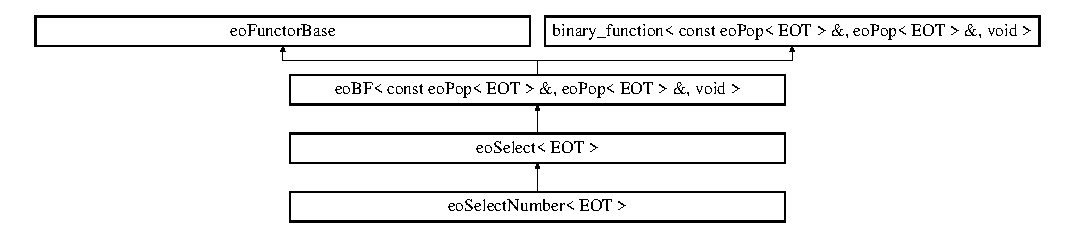
\includegraphics[height=2.75184cm]{classeo_select_number}
\end{center}
\end{figure}
\subsection*{Public Member Functions}
\begin{CompactItemize}
\item 
{\bf eo\-Select\-Number} ({\bf eo\-Select\-One}$<$ {\bf EOT} $>$ \&\_\-select, unsigned \_\-nb\_\-to\_\-select=1)\label{classeo_select_number_a0}

\begin{CompactList}\small\item\em init \item\end{CompactList}\item 
virtual void {\bf operator()} (const {\bf eo\-Pop}$<$ {\bf EOT} $>$ \&\_\-source, {\bf eo\-Pop}$<$ {\bf EOT} $>$ \&\_\-dest)
\begin{CompactList}\small\item\em The implementation repeatidly selects an individual. \item\end{CompactList}\end{CompactItemize}
\subsection*{Private Attributes}
\begin{CompactItemize}
\item 
{\bf eo\-Select\-One}$<$ {\bf EOT} $>$ \& {\bf select}\label{classeo_select_number_r0}

\item 
unsigned {\bf nb\_\-to\_\-select}\label{classeo_select_number_r1}

\end{CompactItemize}


\subsection{Detailed Description}
\subsubsection*{template$<$class EOT$>$ class eo\-Select\-Number$<$ EOT $>$}

eo\-Select\-Number selects many individuals using {\bf eo\-Select\-One}{\rm (p.\,\pageref{classeo_select_one})} as it's mechanism. 

Therefore eo\-Select\-Number needs an {\bf eo\-Select\-One}{\rm (p.\,\pageref{classeo_select_one})} in its ctor

It will select a fixed number of individuals and pushes them to the back of the destination population. 



Definition at line 42 of file eo\-Select\-Number.h.

\subsection{Member Function Documentation}
\index{eoSelectNumber@{eo\-Select\-Number}!operator()@{operator()}}
\index{operator()@{operator()}!eoSelectNumber@{eo\-Select\-Number}}
\subsubsection{\setlength{\rightskip}{0pt plus 5cm}template$<$class EOT$>$ virtual void {\bf eo\-Select\-Number}$<$ {\bf EOT} $>$::operator() (const {\bf eo\-Pop}$<$ {\bf EOT} $>$ \& {\em \_\-source}, {\bf eo\-Pop}$<$ {\bf EOT} $>$ \& {\em \_\-dest})\hspace{0.3cm}{\tt  [inline, virtual]}}\label{classeo_select_number_a1}


The implementation repeatidly selects an individual. 

\begin{Desc}
\item[Parameters:]
\begin{description}
\item[{\em \_\-source}]the source population \item[{\em \_\-dest}]the resulting population (size of this population is the number of times {\bf eo\-Select\-One}{\rm (p.\,\pageref{classeo_select_one})} is called. It empties the destination and adds the selection into it) \end{description}
\end{Desc}


Implements {\bf eo\-BF$<$ const eo\-Pop$<$ EOT $>$ \&, eo\-Pop$<$ EOT $>$ \&, void $>$} {\rm (p.\,\pageref{classeo_b_f_a1})}.

Definition at line 55 of file eo\-Select\-Number.h.

References eo\-Select\-One$<$ EOT, Worth\-T $>$::setup().

The documentation for this class was generated from the following file:\begin{CompactItemize}
\item 
eo\-Select\-Number.h\end{CompactItemize}
